\documentclass[twoside]{book}

% Packages required by doxygen
\usepackage{fixltx2e}
\usepackage{calc}
\usepackage{doxygen}
\usepackage[export]{adjustbox} % also loads graphicx
\usepackage{graphicx}
\usepackage[utf8]{inputenc}
\usepackage{makeidx}
\usepackage{multicol}
\usepackage{multirow}
\PassOptionsToPackage{warn}{textcomp}
\usepackage{textcomp}
\usepackage[nointegrals]{wasysym}
\usepackage[table]{xcolor}

% Font selection
\usepackage[T1]{fontenc}
\usepackage[scaled=.90]{helvet}
\usepackage{courier}
\usepackage{amssymb}
\usepackage{sectsty}
\renewcommand{\familydefault}{\sfdefault}
\allsectionsfont{%
  \fontseries{bc}\selectfont%
  \color{darkgray}%
}
\renewcommand{\DoxyLabelFont}{%
  \fontseries{bc}\selectfont%
  \color{darkgray}%
}
\newcommand{\+}{\discretionary{\mbox{\scriptsize$\hookleftarrow$}}{}{}}

% Page & text layout
\usepackage{geometry}
\geometry{%
  a4paper,%
  top=2.5cm,%
  bottom=2.5cm,%
  left=2.5cm,%
  right=2.5cm%
}
\tolerance=750
\hfuzz=15pt
\hbadness=750
\setlength{\emergencystretch}{15pt}
\setlength{\parindent}{0cm}
\setlength{\parskip}{3ex plus 2ex minus 2ex}
\makeatletter
\renewcommand{\paragraph}{%
  \@startsection{paragraph}{4}{0ex}{-1.0ex}{1.0ex}{%
    \normalfont\normalsize\bfseries\SS@parafont%
  }%
}
\renewcommand{\subparagraph}{%
  \@startsection{subparagraph}{5}{0ex}{-1.0ex}{1.0ex}{%
    \normalfont\normalsize\bfseries\SS@subparafont%
  }%
}
\makeatother

% Headers & footers
\usepackage{fancyhdr}
\pagestyle{fancyplain}
\fancyhead[LE]{\fancyplain{}{\bfseries\thepage}}
\fancyhead[CE]{\fancyplain{}{}}
\fancyhead[RE]{\fancyplain{}{\bfseries\leftmark}}
\fancyhead[LO]{\fancyplain{}{\bfseries\rightmark}}
\fancyhead[CO]{\fancyplain{}{}}
\fancyhead[RO]{\fancyplain{}{\bfseries\thepage}}
\fancyfoot[LE]{\fancyplain{}{}}
\fancyfoot[CE]{\fancyplain{}{}}
\fancyfoot[RE]{\fancyplain{}{\bfseries\scriptsize Generated by Doxygen }}
\fancyfoot[LO]{\fancyplain{}{\bfseries\scriptsize Generated by Doxygen }}
\fancyfoot[CO]{\fancyplain{}{}}
\fancyfoot[RO]{\fancyplain{}{}}
\renewcommand{\footrulewidth}{0.4pt}
\renewcommand{\chaptermark}[1]{%
  \markboth{#1}{}%
}
\renewcommand{\sectionmark}[1]{%
  \markright{\thesection\ #1}%
}

% Indices & bibliography
\usepackage{natbib}
\usepackage[titles]{tocloft}
\setcounter{tocdepth}{3}
\setcounter{secnumdepth}{5}
\makeindex

% Hyperlinks (required, but should be loaded last)
\usepackage{ifpdf}
\ifpdf
  \usepackage[pdftex,pagebackref=true]{hyperref}
\else
  \usepackage[ps2pdf,pagebackref=true]{hyperref}
\fi
\hypersetup{%
  colorlinks=true,%
  linkcolor=blue,%
  citecolor=blue,%
  unicode%
}

% Custom commands
\newcommand{\clearemptydoublepage}{%
  \newpage{\pagestyle{empty}\cleardoublepage}%
}

\usepackage{caption}
\captionsetup{labelsep=space,justification=centering,font={bf},singlelinecheck=off,skip=4pt,position=top}

%===== C O N T E N T S =====

\begin{document}

% Titlepage & ToC
\hypersetup{pageanchor=false,
             bookmarksnumbered=true,
             pdfencoding=unicode
            }
\pagenumbering{roman}
\begin{titlepage}
\vspace*{7cm}
\begin{center}%
{\Large Doxy\+Test \\[1ex]\large 1.\+0 }\\
\vspace*{1cm}
{\large Generated by Doxygen 1.8.11}\\
\end{center}
\end{titlepage}
\clearemptydoublepage
\tableofcontents
\clearemptydoublepage
\pagenumbering{arabic}
\hypersetup{pageanchor=true}

%--- Begin generated contents ---
\chapter{doxy\+Test}
\label{md__home_travis_build_S14P_doxyTest_README}
\hypertarget{md__home_travis_build_S14P_doxyTest_README}{}
\input{md__home_travis_build_S14P_doxyTest_README}
\chapter{Class Index}
\section{Class List}
Here are the classes, structs, unions and interfaces with brief descriptions\+:\begin{DoxyCompactList}
\item\contentsline{section}{\hyperlink{classmy_class}{my\+Class} }{\pageref{classmy_class}}{}
\end{DoxyCompactList}

\chapter{File Index}
\section{File List}
Here is a list of all files with brief descriptions\+:\begin{DoxyCompactList}
\item\contentsline{section}{/home/travis/build/\+S14\+P/doxy\+Test/\hyperlink{main_8cpp}{main.\+cpp} }{\pageref{main_8cpp}}{}
\item\contentsline{section}{/home/travis/build/\+S14\+P/doxy\+Test/\hyperlink{my_class_8cpp}{my\+Class.\+cpp} }{\pageref{my_class_8cpp}}{}
\item\contentsline{section}{/home/travis/build/\+S14\+P/doxy\+Test/\hyperlink{my_class_8h}{my\+Class.\+h} }{\pageref{my_class_8h}}{}
\end{DoxyCompactList}

\chapter{Class Documentation}
\hypertarget{classmy_class}{}\section{my\+Class Class Reference}
\label{classmy_class}\index{my\+Class@{my\+Class}}


{\ttfamily \#include $<$my\+Class.\+h$>$}

\subsection*{Public Member Functions}
\begin{DoxyCompactItemize}
\item 
\hyperlink{classmy_class_aa9e6b37bebb590a0d6aebdb165e308bc}{my\+Class} ()
\item 
\hyperlink{classmy_class_a14f71b961aa14a651c1838ad950218dc}{myfunction} ()
\end{DoxyCompactItemize}


\subsection{Constructor \& Destructor Documentation}
\index{my\+Class@{my\+Class}!my\+Class@{my\+Class}}
\index{my\+Class@{my\+Class}!my\+Class@{my\+Class}}
\subsubsection[{\texorpdfstring{my\+Class()}{myClass()}}]{\setlength{\rightskip}{0pt plus 5cm}my\+Class\+::my\+Class (
\begin{DoxyParamCaption}
{}
\end{DoxyParamCaption}
)}\hypertarget{classmy_class_aa9e6b37bebb590a0d6aebdb165e308bc}{}\label{classmy_class_aa9e6b37bebb590a0d6aebdb165e308bc}


\subsection{Member Function Documentation}
\index{my\+Class@{my\+Class}!myfunction@{myfunction}}
\index{myfunction@{myfunction}!my\+Class@{my\+Class}}
\subsubsection[{\texorpdfstring{myfunction()}{myfunction()}}]{\setlength{\rightskip}{0pt plus 5cm}my\+Class\+::myfunction (
\begin{DoxyParamCaption}
{}
\end{DoxyParamCaption}
)}\hypertarget{classmy_class_a14f71b961aa14a651c1838ad950218dc}{}\label{classmy_class_a14f71b961aa14a651c1838ad950218dc}


The documentation for this class was generated from the following files\+:\begin{DoxyCompactItemize}
\item 
/home/travis/build/\+S14\+P/doxy\+Test/\hyperlink{my_class_8h}{my\+Class.\+h}\item 
/home/travis/build/\+S14\+P/doxy\+Test/\hyperlink{my_class_8cpp}{my\+Class.\+cpp}\end{DoxyCompactItemize}

\chapter{File Documentation}
\hypertarget{main_8cpp}{}\section{/home/travis/build/\+S14\+P/doxy\+Test/main.cpp File Reference}
\label{main_8cpp}\index{/home/travis/build/\+S14\+P/doxy\+Test/main.\+cpp@{/home/travis/build/\+S14\+P/doxy\+Test/main.\+cpp}}
{\ttfamily \#include \char`\"{}my\+Class.\+h\char`\"{}}\\*
Include dependency graph for main.\+cpp\+:
\nopagebreak
\begin{figure}[H]
\begin{center}
\leavevmode
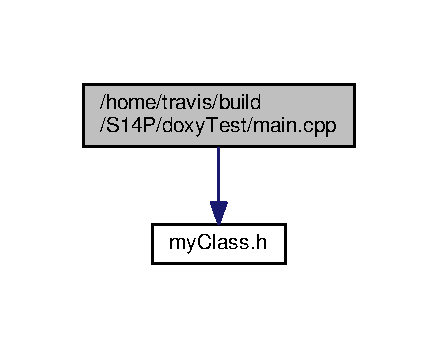
\includegraphics[width=210pt]{main_8cpp__incl}
\end{center}
\end{figure}
\subsection*{Functions}
\begin{DoxyCompactItemize}
\item 
int \hyperlink{main_8cpp_ae66f6b31b5ad750f1fe042a706a4e3d4}{main} ()
\end{DoxyCompactItemize}


\subsection{Function Documentation}
\index{main.\+cpp@{main.\+cpp}!main@{main}}
\index{main@{main}!main.\+cpp@{main.\+cpp}}
\subsubsection[{\texorpdfstring{main()}{main()}}]{\setlength{\rightskip}{0pt plus 5cm}int main (
\begin{DoxyParamCaption}
{}
\end{DoxyParamCaption}
)}\hypertarget{main_8cpp_ae66f6b31b5ad750f1fe042a706a4e3d4}{}\label{main_8cpp_ae66f6b31b5ad750f1fe042a706a4e3d4}

\hypertarget{my_class_8cpp}{}\section{/home/travis/build/\+S14\+P/doxy\+Test/my\+Class.cpp File Reference}
\label{my_class_8cpp}\index{/home/travis/build/\+S14\+P/doxy\+Test/my\+Class.\+cpp@{/home/travis/build/\+S14\+P/doxy\+Test/my\+Class.\+cpp}}
{\ttfamily \#include \char`\"{}my\+Class.\+h\char`\"{}}\\*
{\ttfamily \#include $<$iostream$>$}\\*
Include dependency graph for my\+Class.\+cpp\+:
\nopagebreak
\begin{figure}[H]
\begin{center}
\leavevmode
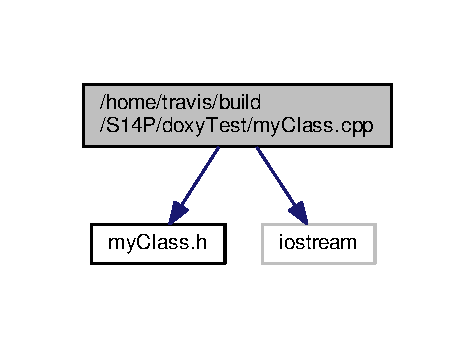
\includegraphics[width=228pt]{my_class_8cpp__incl}
\end{center}
\end{figure}

\hypertarget{my_class_8h}{}\section{/home/travis/build/\+S14\+P/doxy\+Test/my\+Class.h File Reference}
\label{my_class_8h}\index{/home/travis/build/\+S14\+P/doxy\+Test/my\+Class.\+h@{/home/travis/build/\+S14\+P/doxy\+Test/my\+Class.\+h}}
This graph shows which files directly or indirectly include this file\+:
\nopagebreak
\begin{figure}[H]
\begin{center}
\leavevmode
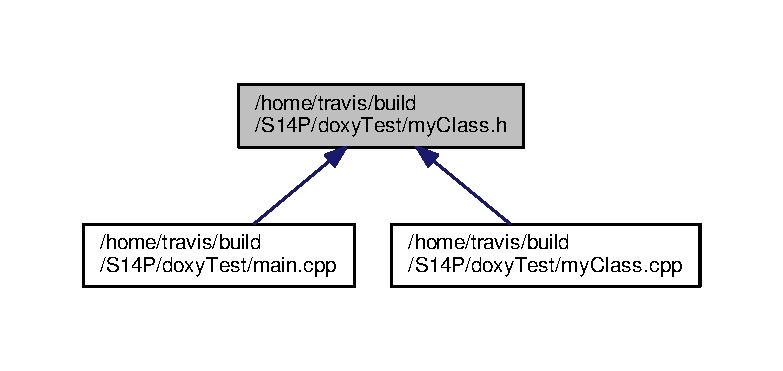
\includegraphics[width=350pt]{my_class_8h__dep__incl}
\end{center}
\end{figure}
\subsection*{Classes}
\begin{DoxyCompactItemize}
\item 
class \hyperlink{classmy_class}{my\+Class}
\end{DoxyCompactItemize}

\hypertarget{_r_e_a_d_m_e_8md}{}\section{/home/travis/build/\+S14\+P/doxy\+Test/\+R\+E\+A\+D\+ME.md File Reference}
\label{_r_e_a_d_m_e_8md}\index{/home/travis/build/\+S14\+P/doxy\+Test/\+R\+E\+A\+D\+M\+E.\+md@{/home/travis/build/\+S14\+P/doxy\+Test/\+R\+E\+A\+D\+M\+E.\+md}}

%--- End generated contents ---

% Index
\backmatter
\newpage
\phantomsection
\clearemptydoublepage
\addcontentsline{toc}{chapter}{Index}
\printindex

\end{document}
